\section{Introduction}

Experiment 12-06-109 (together with E12-09-007b) is a comprehensive program to map out the $x$- and $Q^2$-dependence of the helicity structure of the nucleon in the region of moderate to very large $x$. By collecting inclusive (DIS) and semi-inclusive (SIDIS) data over a wide kinematic range with CLAS12 and 11 GeV polarized electrons on both longitudinally polarized protons (NH$_3$) and deuterons (ND$_3$), this program aims to constrain global fits of polarized parton (quark and gluon) distributions, extract higher twist corrections to the DIS structure functions, and evaluate moments connected to local operators in the Operator Product Expansion (OPE). 
Experiment 12-06-109 was originally approved by PAC 30 (with a further review and scientific rating of ``A'' by PAC 36) for a total of 80 days, 30 days on NH$_3$ and 50 days on ND$_3$ (both including overhead).

In the meantime, additional experiments~\cite{RGC} on longitudinally polarized {\em protons} have been approved, with high rating. These experiments have brought the total number of PAC-approved days for the NH$_3$ target to 120 (run group Ca with CLAS12). 
In the meantime, the total runtime for the ND$_3$ target (run group Cb) has been largely unchanged (at present 65 days including all overhead for auxiliary measurements, target operations etc.). This discrepancy is even more striking when taking into account that ND$_3$ targets tend to have polarizations of roughly a factor 1/2 lower than NH$_3$ targets, resulting in an overall figure of merit (FoM) at least four times worse than for the proton. This means that any  analysis that requires information from both targets (e.g., global fits to extract polarized parton distributions) would have uncertainties that are totally dominated by the statistical error from the deuteron.

While some of the goals of the original experiment 12-06-109 can be reached with reasonable precision even with 50 PAC days on the deuteron, there are some physics observables whose precision would be ``statistics-starved'' under this scenario. In particular, the asymptotic behavior of the PDF $\Delta d$ at large $x$ would be much less constrained than what is possible with a doubling of the integrated luminosity. Deuteron data are also crucial to determine the total contribution from quark helicities to the nucleon spin ($\Delta \Sigma$), as well as polarized gluon and strange quark PDFs at moderate to large $x$ (see details in the following sections). Because of their smaller count rates, SIDIS channels will benefit significantly from additional statistics. As we lay out in detail in the following sections, a doubling of the actual run time on polarized ND$_3$ from 50 to 100 days (plus the necessary overhead) will optimize the overall physics output from Experiment 12-06-109 and maximize the return on the large investment in the spin physics program with Jefferson Lab at 12 GeV.
No other facility presently running or under construction will be able to probe, with comparable precision, the kinematic region of moderate to large $x$ and moderate $Q^2$ accessible here.

%The additional 10 days at 5 nA with the inclusion of the Forward Tagger, as requested in the nDVCS part of this proposal, will not directly impact the program of measuring collinear spin structure functions, and has not been included in the estimates that follow in this chapter. However, it offers the potential for measurements of spin structure functions at very low $Q^2$ (measuring the scattered electron in the FT), that are of interest in their own right, and as part of the radiative corrections for DIS. 

%To fully elucidate the spin structure of the nucleon in the valence region, one has to combine 
%information from many different experimental approaches. Both deeply virtual exclusive processes,
%which are sensitive to Generalized Parton Distributions (GPDs), and semi-inclusive processes (in particular
%those involving single spin asymmetries which are sensitive to Transverse Momentum-dependent Distributions - TMDs)
% will access some part of this puzzle. However, high precision
%measurements of structure functions (as well as of elastic form factors) remain indispensable, both to
%constrain the parameters of GPD and TMD fits, and as the most direct access to the longitudinal structure
%of the nucleon. In particular, spin structure functions of the nucleon in the valence region and at very large
%$x$ are still poorly known, in spite of their fundamental significance for tests of pQCD and models of
%nucleon structure. Jefferson Lab with 11-12 GeV beams is the unique place where this gap can be finally closed.
%The accessible kinematics is also uniquely suited to study the transition from partonic degrees of freedom
%to hadronic ones, through detailed measurements of higher twist operator matrix elements and a
%complete investigation of the phenomenon of quark-hadron duality in spin structure functions.

\subsection{The Deuteron and CLAS12}

A complete mapping of spin structure functions and the extraction, through global PDF fits, of polarized parton distributions require a complete set of measurements on both types of nucleons, protons and neutrons, over the widest possible range in $x$ and $Q^2$. 
In addition, since neutrons can only be accessed bound in nuclei, it is very important that both commonly used nuclear targets, $^3$He and deuterium, be studied with high precision, since nuclear effects and their uncertainties are very different for these two cases. Furthermore, the deuteron is the best substitute for a purely isoscalar nucleon target, which is ideal for extracting information on gluon and sea quark helicity distributions through NLO analyses. For these reasons, a high-statistics measurement on polarized deuterium (ND$_3$) is obligatory.

Presently, the only readily available and suitable targets for polarized protons and deuterons employ solid state compounds like ammonia, butanol or lithium deuteride at low ($\approx 1$ K) temperatures. 
These compounds are susceptible to radiation damage and beam heating, limiting severely the practically achievable luminosities. 
The upgraded CLAS12 detector will be a perfect match for these targets, since it
\begin{itemize}
\item is optimized for luminosities of 1-2$\cdot 10^{35}$ cm$^{-2}$ s$^{-1}$, within a factor of 2-4 of the practical limit of cryogenic ammonia targets, and compensates for this relatively low luminosity with its very large acceptance
\item already contains a solenoidal magnet which will provide the (typically 5 Tesla) field needed for dynamic nuclear polarization, thus minimizing the extra costs of a polarized target
\item covers a large angular range, including backwards angles, which allows us to simultaneously measure inclusive, semi-inclusive and tagged structure functions (with backward-going target remnants) over the full kinematic range of interest (while also collecting data for deeply virtual exclusive processes and single spin asymmetries).
\end{itemize}

Our group is leading the development of an optimized longitudinally polarized proton and deuteron target for CLAS12, and coordinates the run group C using these targets. Significant investments in this program have already been made, partially through an NSF MRI grant. No other experiment with this particular type of targets has been planned with similar kinematics, at Jefferson Lab or elsewhere. We believe that adding 50 more days of running, plus overhead, to the already established run group C (an overall increase by only 25\%) will yield an optimal return on this investment.

\section{Scientific Case and Recent Developments}

\begin{figure}[htb!]
\begin{center}
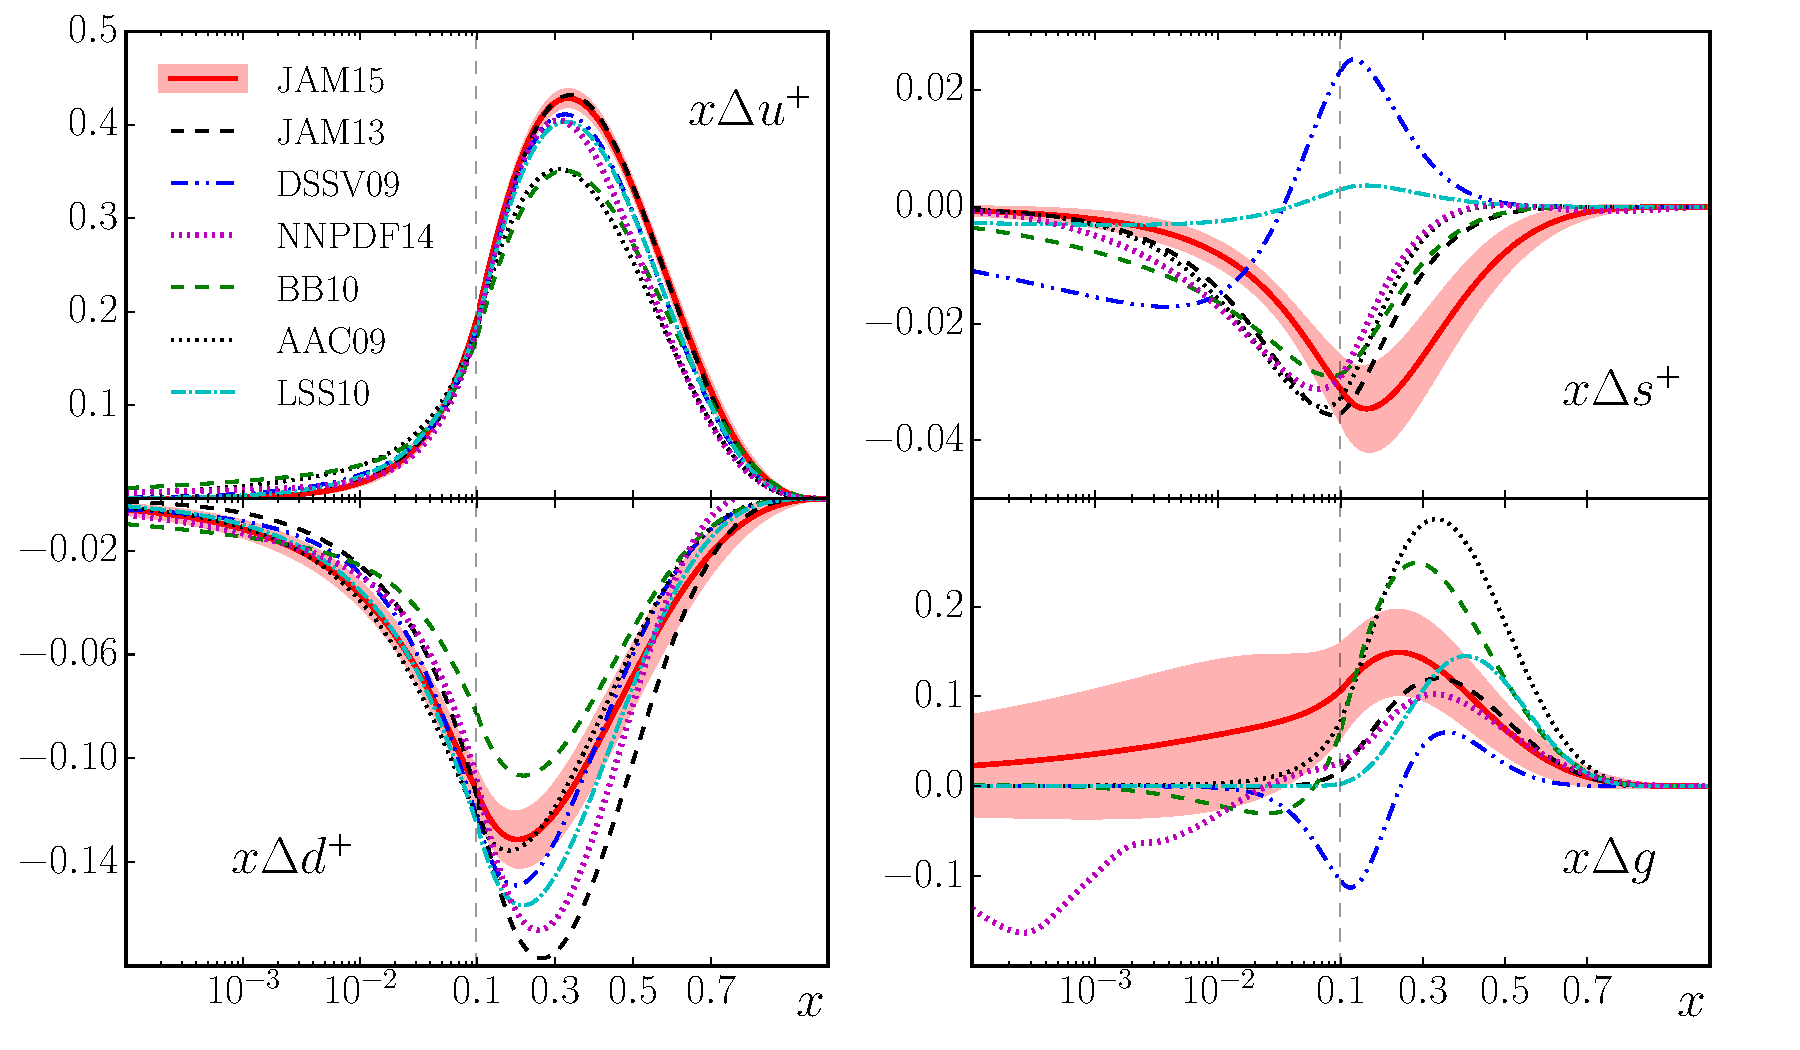
\includegraphics[width=6in]{dis/LT_all_groups.pdf}
\end{center}
\caption{\baselineskip 13pt \small
Compilation of recent  polarized PDF fits from various groups. This Figure is from the  JAM15 paper~\cite{JAM15}
(Fig. 17) where all references for these fits can be found.}
\label{NLOfits}
\end{figure}

Inclusive and flavor-tagged spin structure functions of the nucleon have been measured for  over three decades~\cite{Kuhn:2008sy}, beginning with the
experiments at SLAC~\cite{Alguard:1976bm} and the discovery of the famous ``spin puzzle'' by the 
EMC~\cite{EMCfinal}. The goal of these experiments is to determine, via next-to-leading-order DGLAP analyses, 
 the helicity-dependent distribution functions (PDFs)
 of valence and sea quarks as well as gluons, see Fig.~\ref{NLOfits}. Collinear spin structure functions can also be used to evaluate 
 moments that are related to nucleon axial current matrix elements (e.g., the overall contribution of quark helicities to the
 nucleon spin), and to test fundamental sum rules like the Bj\"orken sum rule~\cite{Bjorken:1968dy}. 
 Finally, measuring their dependence on the
 photon virtuality $Q^2$ allows us to determine higher twist contributions, matrix elements in the framework of the operator
 product expansion (OPE), and the transition from partonic (high $Q^2$) to hadronic (low $Q^2$) degrees of freedom,
 including duality and 
 tests of the Gerasimov-Drell-Hearn sum rule and its extensions in, e.g., Chiral perturbation theory (see
 discussion and references in~\cite{Kuhn:2008sy}).
 In the new era of three-dimensional mapping of the nucleon parton distributions, collinear spin structure functions
 serve both as a crucial constraint on GPDs and TMDs, and provide two of the four ingredients to the celebrated
 nucleon spin sum rule.
 
Within recent years, data from high-energy polarized proton collisions at 
RHIC~\cite{STAR_jet15,PHENIX_pi14,PHENIX_pi15,STAR_W14,PHENIX_W15} 
have constrained the contribution of gluon
and sea quark helicities at low to moderate $x \le 0.2$ to the nucleon spin. Further information has come from measurements
of open charm production~\cite{COMPASS_g13}. The most recent 
inclusive data from COMPASS~\cite{COMPASS16} extend our knowledge of spin structure functions to the lowest
$x$ and highest $Q^2$ yet. 
Meanwhile, the spin structure function program with Jefferson Lab's 6 GeV has been concluded and most results have been 
published. In particular, very precise data on proton, deuteron and $^3$He 
targets~\cite{eg1b-d,eg1b-p,eg1-dvcs,E06-014_A1,E06-014_d2,E01-012}
 have recently appeared 
that cover a large kinematic range, from low $Q^2$ to the DIS region. This program is being continued in the 12 GeV era, with several
experiments in three halls approved with scientific rating of ``A''. The unique importance of these expected Jefferson Lab 
data is threefold:

\begin{figure}[htb!]
\begin{center}
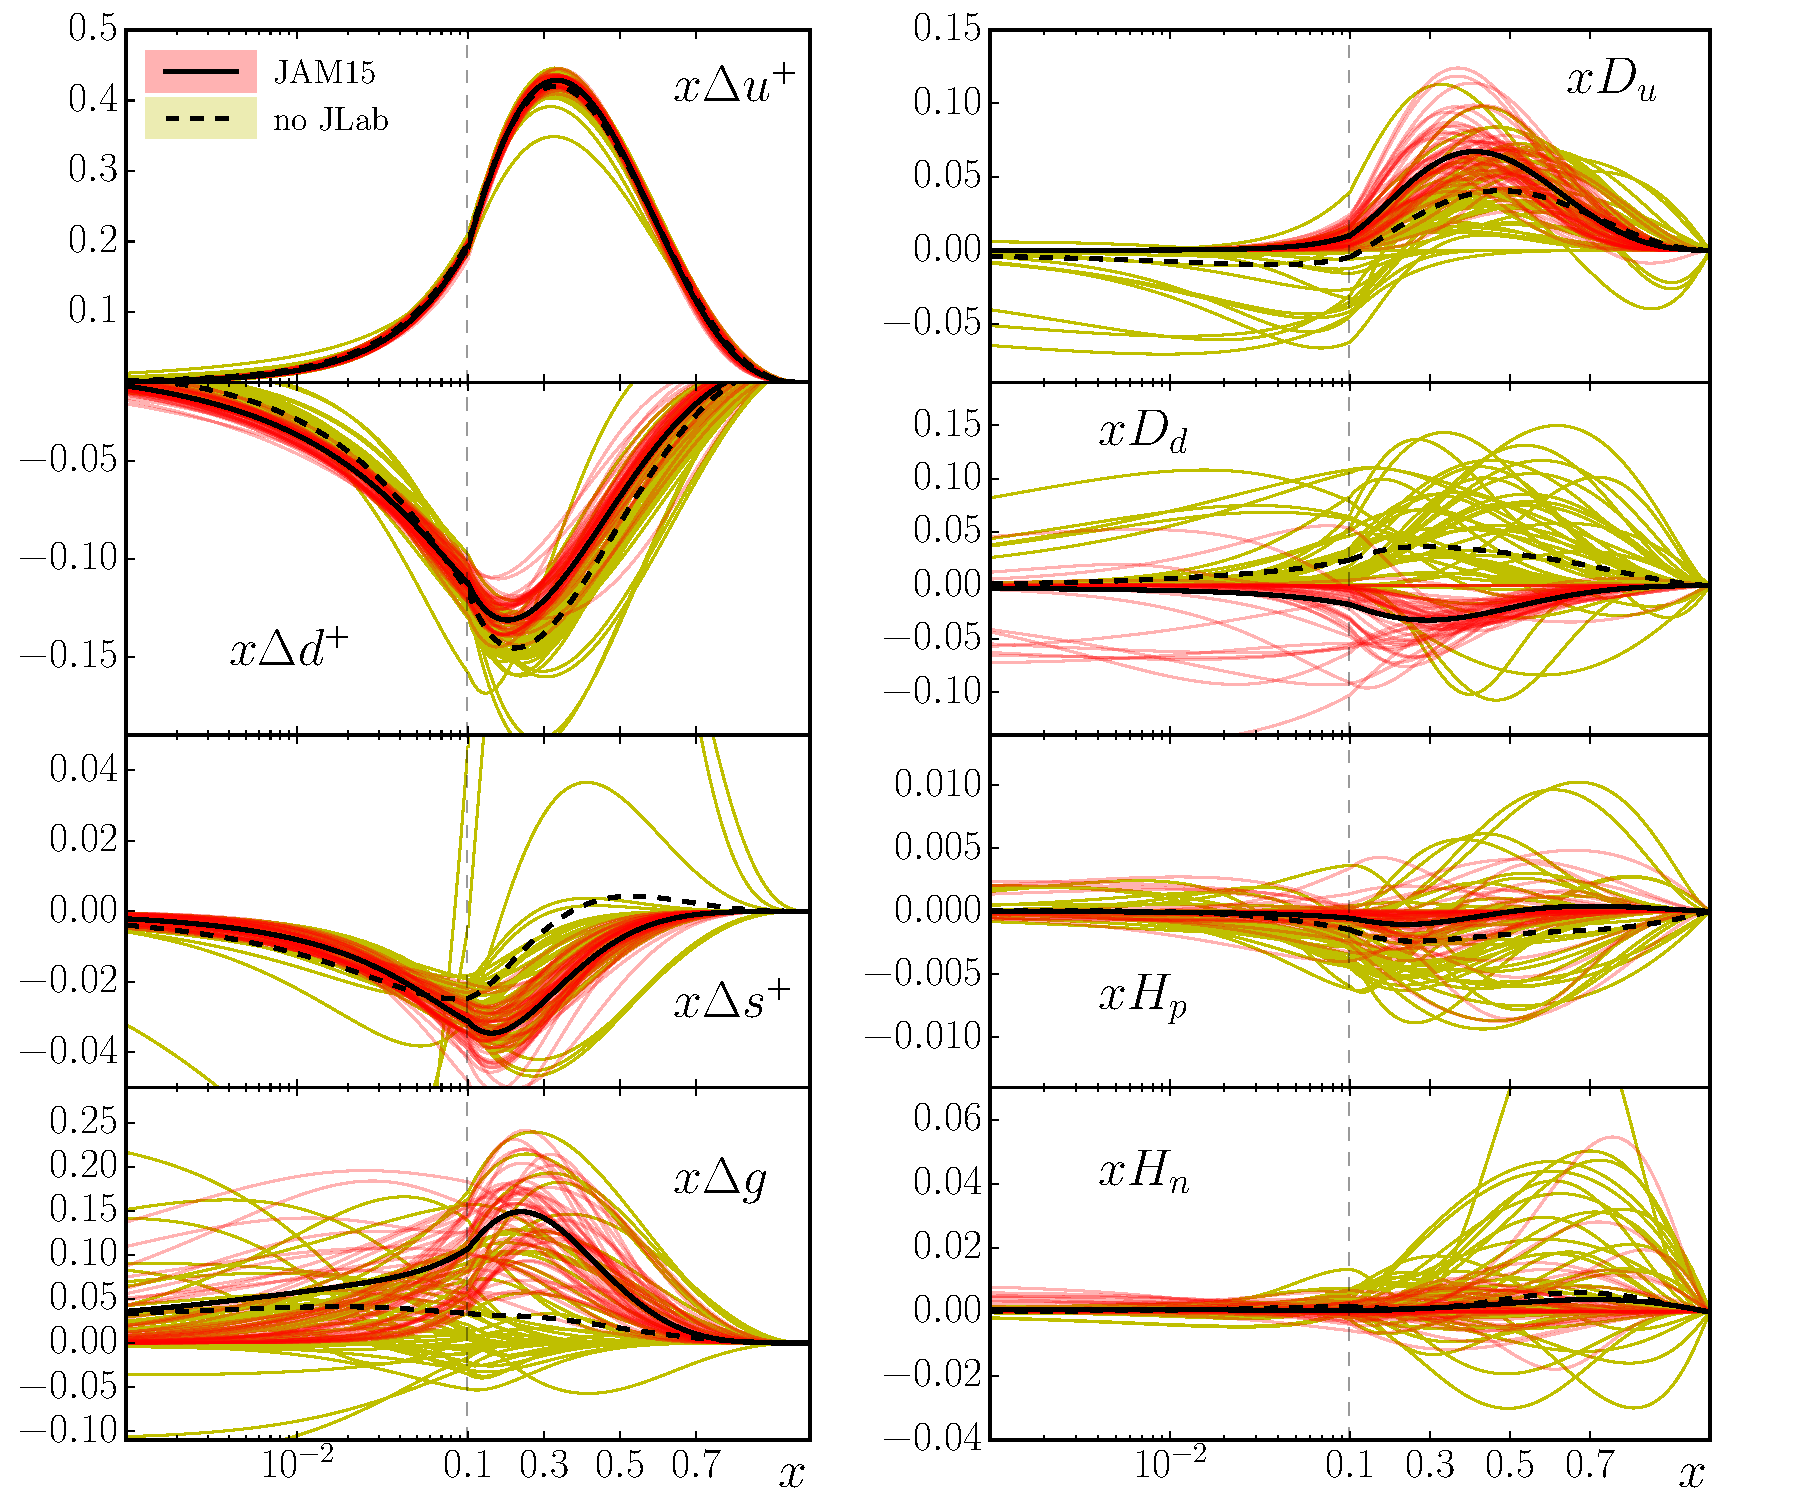
\includegraphics[width=6in]{dis/IMPACT_JLAB.pdf}
\end{center}
\caption{\baselineskip 13pt \small
Impact of recent Jefferson Lab data on the global NLO PDF fit by the Jefferson Lab Angular Momentum (JAM) collaboration. 
This Figure is from the recent JAM15 paper~\cite{JAM15}
(Fig. 15) where all relevant references  can be found. The l.h.s. fits are for the leading twist distributions for three quark flavors
and gluons, while the r.h.s. shows the results for various higher-twist terms.The yellow lines are from repeated
Monte Carlo fits including all world data except those from Jefferson Lab; the red lines include the Jefferson Lab data and
clearly have a much more narrow uncertainty band.}
\label{JLabImpact}
\end{figure}

\begin{enumerate}
\item For a DGLAP determination of all individual parton distribution functions, but in particular those of the gluon, from DIS data,
a large leverarm in $Q^2$ is required to exploit scaling violations. The recent precise data from COMPASS~\cite{COMPASS16}
cover the high-$Q^2$ limit\footnote{These will be greatly improved upon, both in kinematic reach and in precision, by data
to be acquired with the future EIC; however, the low-$Q^2$ data fromJefferson Lab will likely not be matched in the foreseeable future.},
 while precise data at the lowest $Q^2$ consistent with DIS come from Jefferson Lab. The latter cover 
a large range in $Q^2$, which in itself allows us to reliably extract and control for higher-twist effects. Figure~\ref{JLabImpact}
demonstrates the significant improvement in our knowledge of {\em all} polarized PDFs enabled already by the existing
Jefferson Lab data.

\begin{figure}[htb!]
\begin{center}
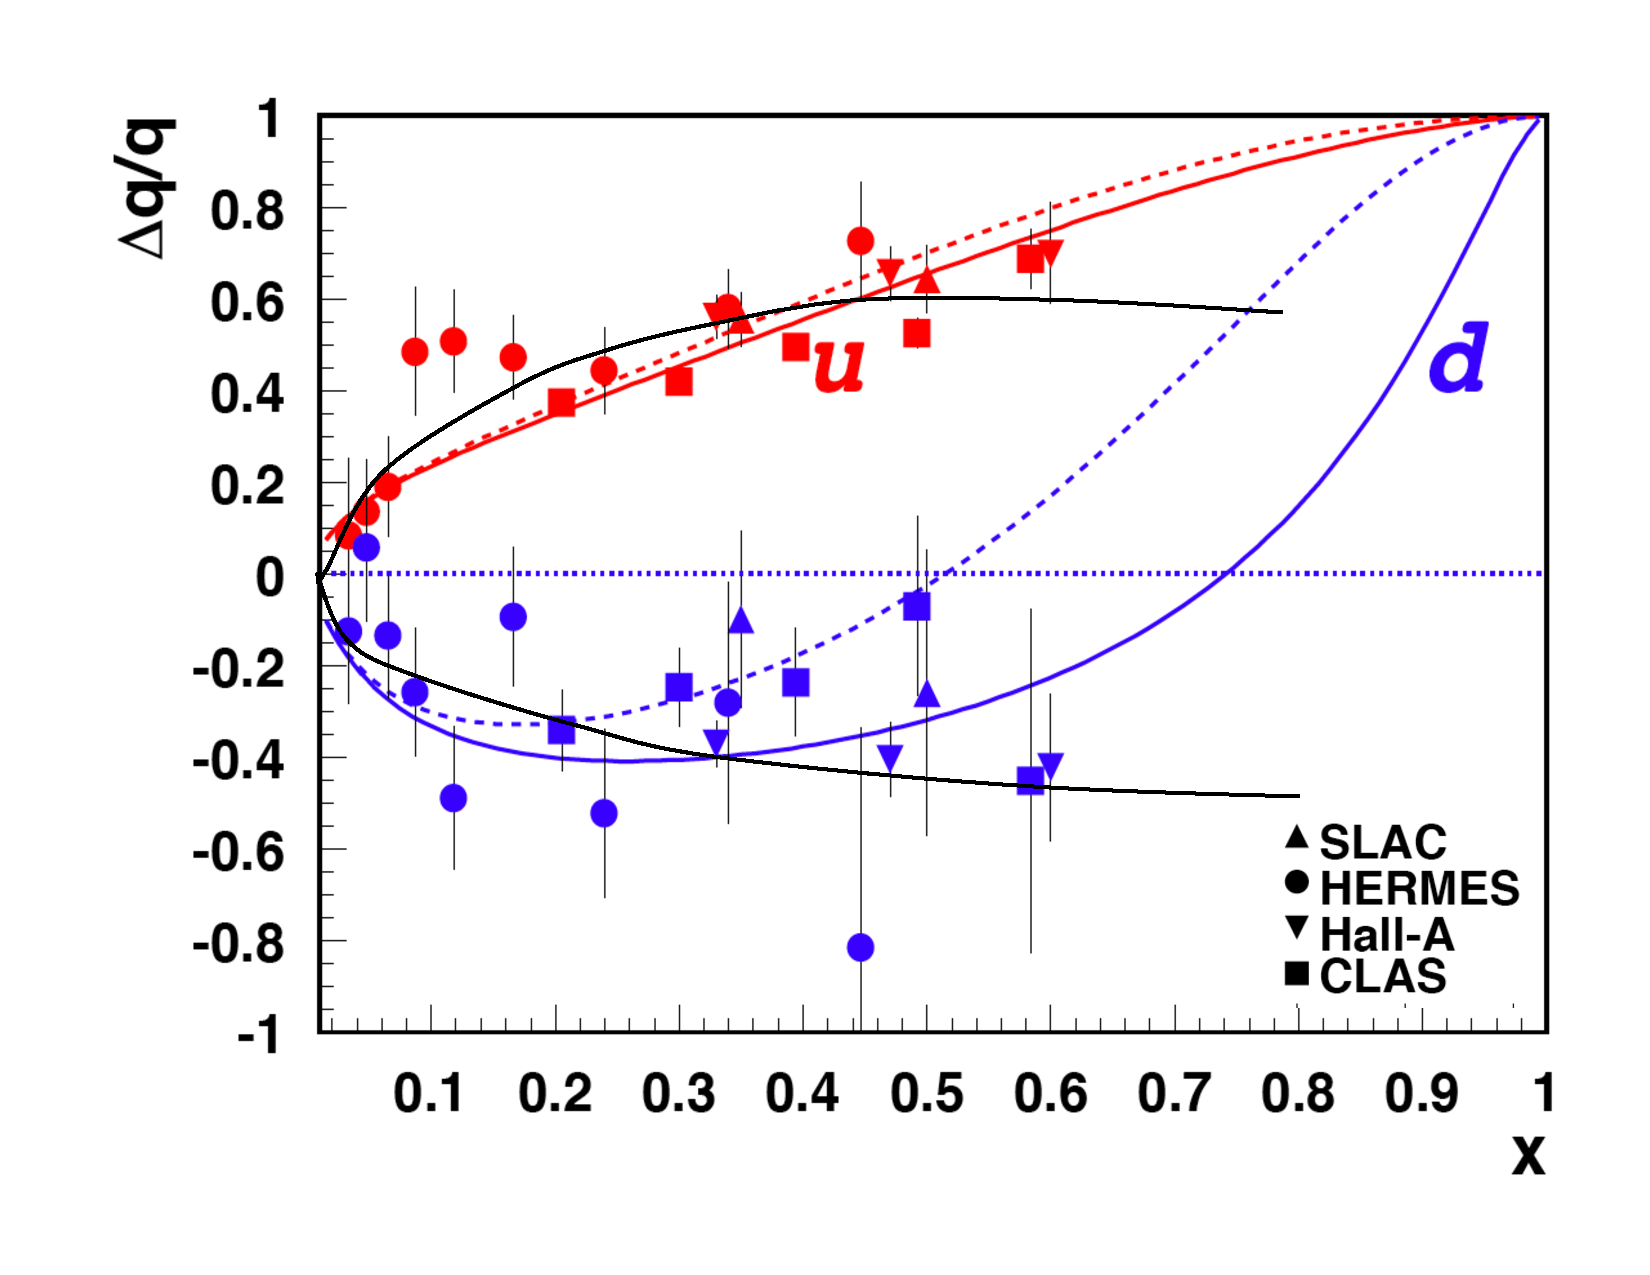
\includegraphics[width=4in]{dis/delqFig-eps-converted-to.pdf}
\end{center}
\vspace{-0.2in}
\caption{\baselineskip 13pt \small
$\Delta u/u$ (upper half) and $\Delta d/d$ (lower half) results from Jefferson Lab
Hall A and CLAS data (in leading order approximation), compared with other world data
and three different predictions: a fit by Leader, Stamenov and Siderov~\cite{Leader:2006xc} (black line), and two pQCD
predictions without~\cite{Brodsky:1994kg} (dashed)  and with~\cite{Avakian:2007xa} (solid red and blue lines)
inclusion of orbital angular momentum effects.  }
\label{highx}
\end{figure}

\item While the contribution from PDFs in the valence region $x > 0.3$ and, especially, in the limit $x \rightarrow 1$, to the overall
nucleon spin is not very large, knowledge of PDFs in this regime is crucial to understand the valence structure of the nucleon and to
test predictions from pQCD and various models. Only Jefferson Lab at 12 GeV can provide the necessary precision data
in these kinematics for the foreseeable future. In particular, the asymptotic polarization of d quarks in the proton,
$\Delta d/ d$ at large $x$, is presently poorly known (see Fig.~\ref{highx}), 
and a reliable measurement requires high statistics data from both
deuterons and $^3$He.

\item Beyond the leading-order PDFs, higher twist structure functions are of high current interest in themselves, since
they contain information about correlations and interactions between gluons and quarks in the nucleon. Again, only at Jefferson Lab, with its unique combination of high luminosity
and moderate $Q^2$, can these structure functions be studied in detail (see
the r.h.s. of  Fig.~\ref{JLabImpact} for
examples).
\end{enumerate}

\begin{figure}[hbt!]
\begin{center}
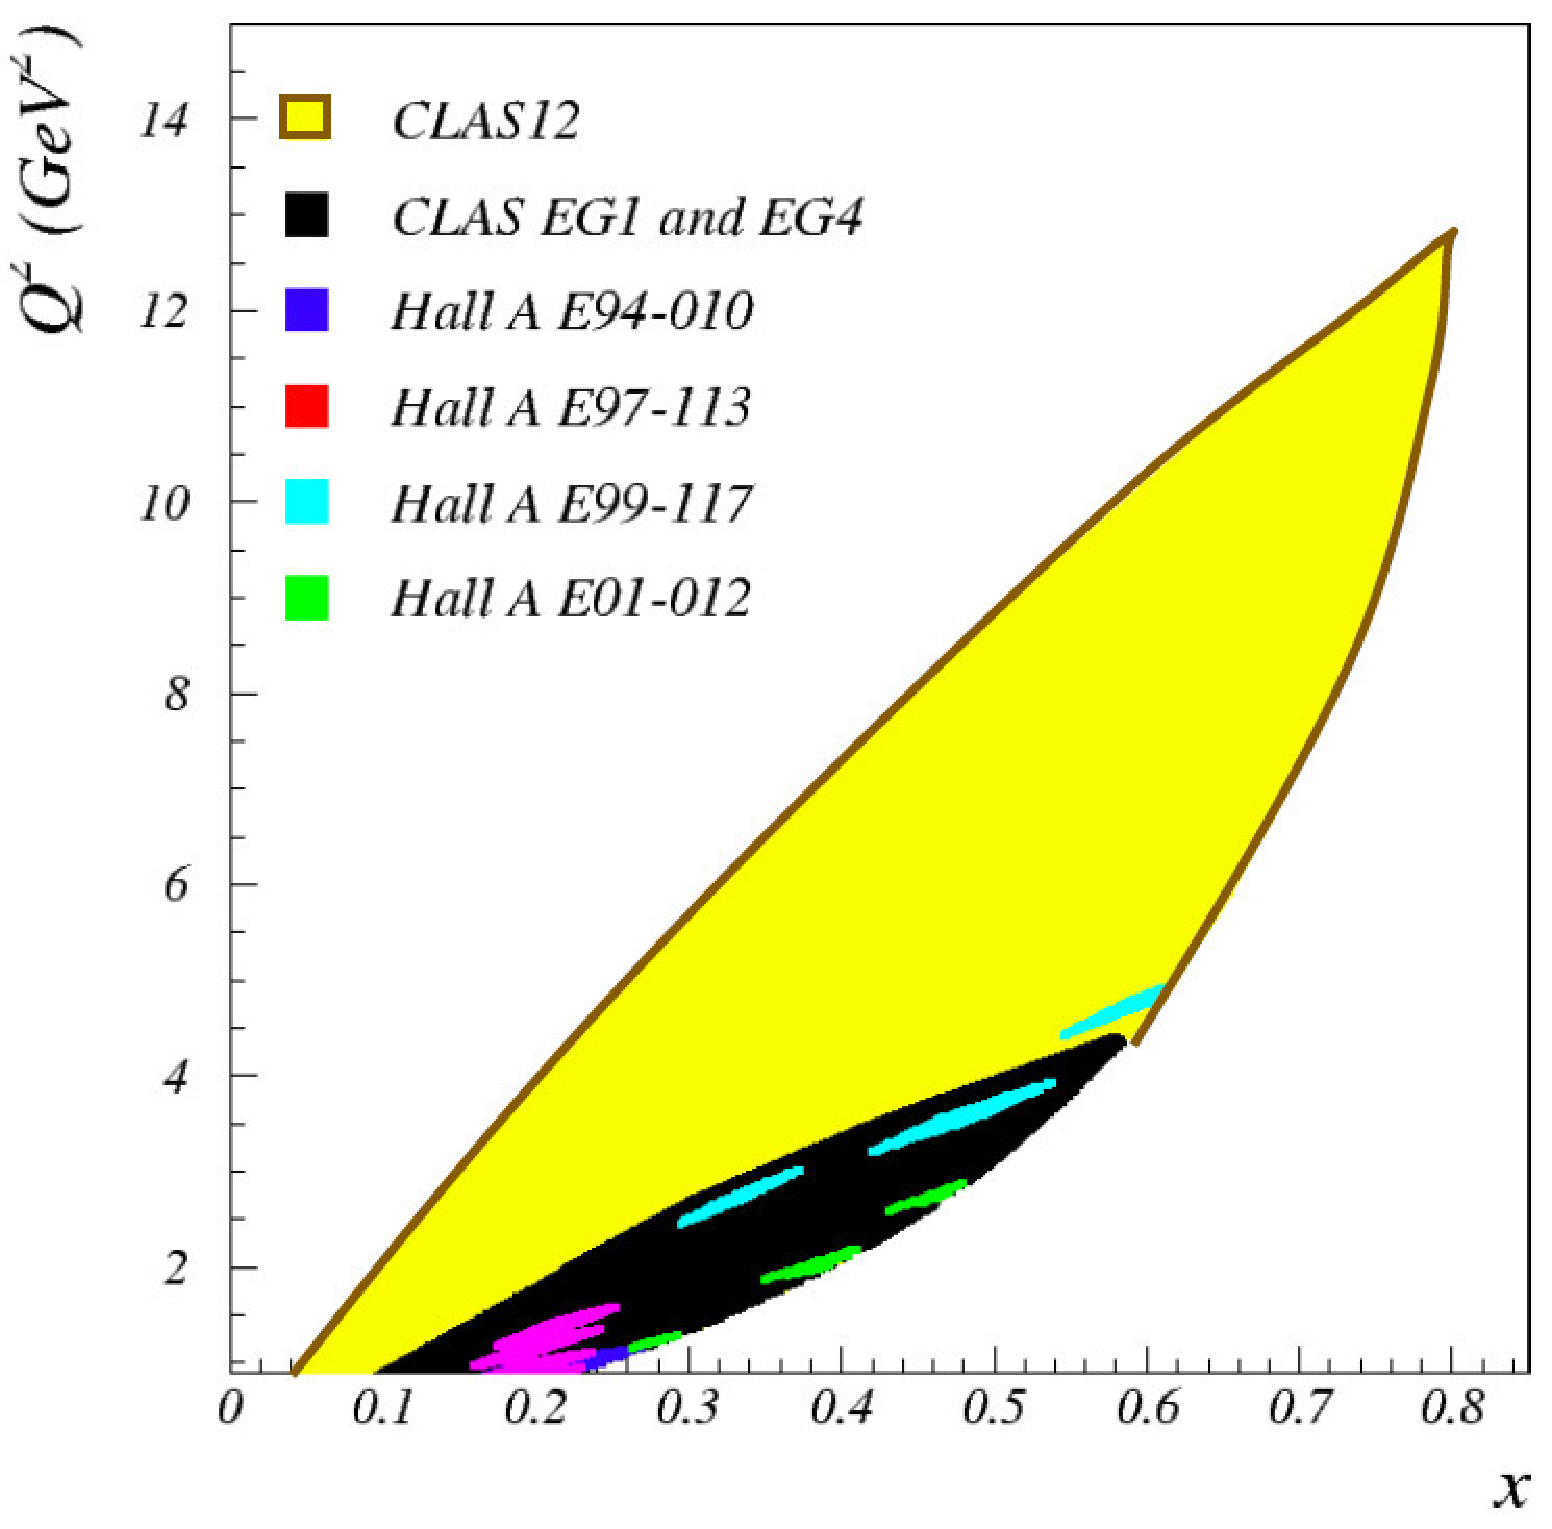
\includegraphics[width=2.5in]{dis/Coverage2-eps-converted-to.pdf}
\end{center}
\caption{\baselineskip 13pt \small
Kinematic coverage in the DIS region
 of existing 6 GeV JLab experiments and expected coverage
for the proposed 12 GeV experiment.}
\label{coverage}
\end{figure}

Experiment 12-06-109 at 11 GeV will 
 extend the useful $x$-range in the DIS region both to lower and
higher $x$ and to much higher $Q^2$, compared to the existing Jefferson Lab data; see Fig.~\ref{coverage}.
Especially at the upper end, the expected data will still be limited in statistics; a doubling of the
integrated luminosity will yield significant improvements in the information we can extract from these data,
as we will show below.

%\section{Technical Progress Towards Realizing the Experiment}
%The proposed experiment will use the standard equipment of CLAS12 in addition to the
%polarized target. Many of the authors on this proposal are actively working on several of the
%detector components of CLAS12, including pre-shower calorimeter, high threshold cherenkov 
%counter,  and Region 1 and 2 forward tracking drift chambers, as well as data analysis software. 
%All of these projects have made significant progress since the experiment was originally approved;
%for example, the first Region 2 drift chamber has been assembled and stringing has begun
%at JLab, with subsequent sectors to be strung in ODU's newly completed clean room.
%
%\begin{figure}[ht]
%%\vspace{-0.2in}
%%\includegraphics[width=12cm, angle=90]{ConceptCutaway1.eps}
%%\vspace{-1in}
%\begin{center}
%\includegraphics[width=6in]{Target.eps}
%\end{center}
%%\centerline{\epsfxsize=6in\epsffile{Target.eps}}
%\caption{\baselineskip 13pt \small
%A schematic drawing of the polarized solid target cryostat and 
%target insert for CLAS12. Note that the required 5 Tesla polarizing magnetic field
%will be provided ``for free'' by the solenoid of the CLAS12 central tracker, which
%was designed with this goal in mind. The target sits inside a horizontal $^4$He
%evaporation refrigerator and will be dynamically polarized using a microwave system. \label {potarg}}
%\end{figure}
%
%The major non-standard item required for successful execution of this program is the polarized target.
%A conceptual design was already completed at the time of the first PAC submission, see Fig.~\ref{potarg}.
%Unfortunately, funding for this target had been 
%subsequently removed from the base equipment budget for the 
%Jefferson Lab 12 GeV upgrade, to cover required contingency costs in other parts of the project.
%In 2009, some of the spokespersons of this experiment (Kuhn, B\"ultmann, Prok, and Crabb) formed
%a consortium and submitted a successful MRI-R$^2$ proposal to NSF. The approved funding from
%this source will cover all costs of acquiring necessary hardware and prototyping, assembly,
%and testing of the polarized target. Subsequent to the availability of these funds, work has begun on
%the detailed design of all target components, in particular the in-beam cryostat and vacuum vessel.
%The design of the central Silicon Vertex Tracker for CLAS12 is now fully consistent with the required
%space to insert the polarized target into its center.
%Initial development work has also begun on the target insert and NMR system; several major components
%and measuring instruments have already been acquired. The total project, which also receives strong
%support from the JLab target group, is on track to be completed within 4 years, making the polarized
%target available as soon as the experimental program with CLAS12 can begin. In addition to the present
%experiment, this target also supports a large (PAC-approved) program of measurements of 
%DVCS (E12-06-119), SIDIS (single target spin asymmetries;  E12-07-107),
% and of the EMC effect in nuclear spin structure functions (LOI 10-005 to PAC35).
%
%At PAC34, a series of SIDIS experiments (Proposals PR12-09-007, 008, 009) were approved for both
%unpolarized and longitudinally polarized target. All of these proposal require a RICH detector (in lieu
%of some sectors of the existing low-threshold cherenkov counter) to separate Kaons from pions
%and protons. Work on the design of such a RICH detector has begun in earnest, and first 
%benchmark results have been presented at CLAS12 workshops. This development will clearly
%benefit the present experiment, as well, as it will allow us to access the full kinematic range of
%flavor-tagged spin structure functions in SIDIS, with separation of all three charge states of pions
%and kaons. This will lead to additional constraints of NLO analyses which will allow us to separate the
%contributions of valence and various sea quarks in the range $x > 0.1$, where existing data
%have relatively large uncertainties and one expects interesting effects to appear (e.g.,
%a possible charge asymmetry in the polarized sea, analog to that seen in unpolarized PDFs).
%Several of the authors of this proposal update are working on this extension of the CLAS12 
%capabilities.

\section{Expected Results}

\subsection{PDFs}

\begin{figure} [!htbp]
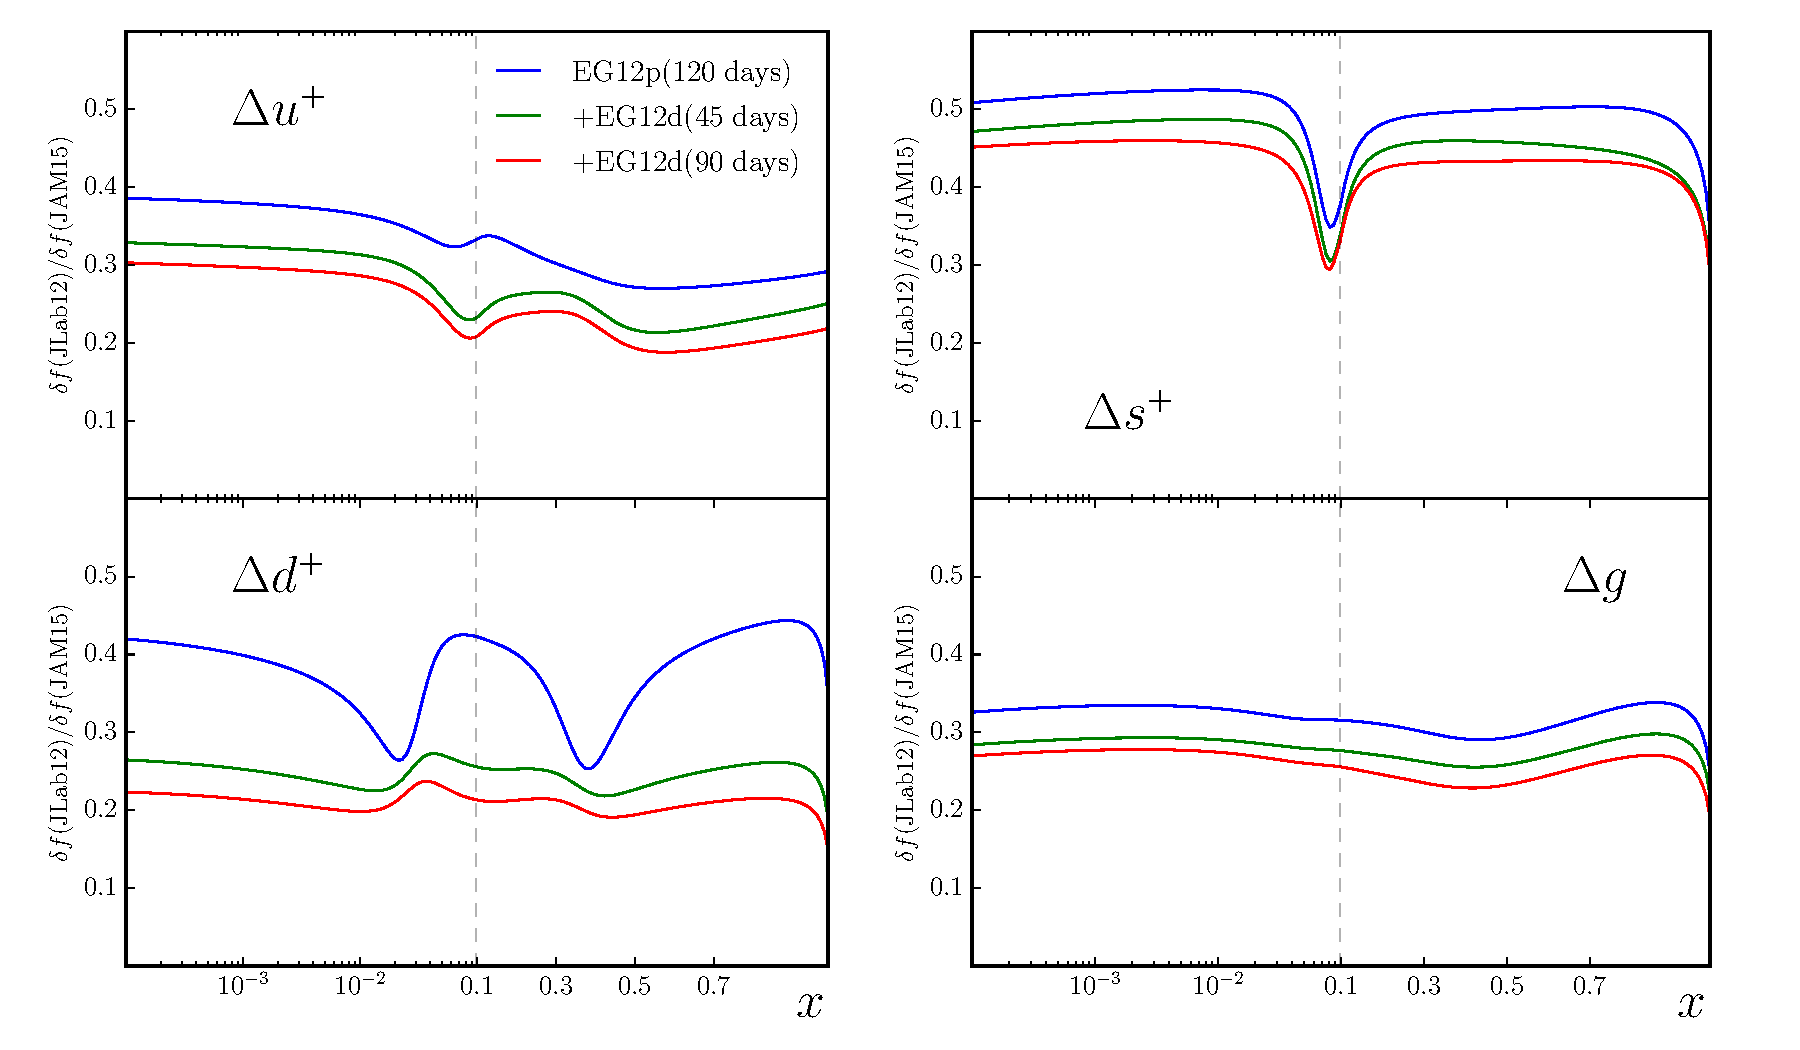
\includegraphics[width=\linewidth]{dis/LTrat.pdf}
\caption{\baselineskip 13pt \small
Expected effect on the uncertainty for various polarized parton distribution
functions after inclusion of E12-06-109 data, according to an up-to-date
analysis by the JAM collaboration (courtesy of N. Sato). 
The blue lines indicate the reduction factor for the present uncertainties (see Fig.~\ref{JLabImpact}) 
from the already approved 120 days of NH$_3$ only, while the green and red lines show the additional reduction from
combining these data with either the already approved 50 days for ND$_3$ (green), or with double that run time (red).}
%PLACEHOLDER: TO BE REPLACED BY UP-TO-DATE JAM RESULTS:
%Expected uncertainties for polarized parton distributions
%$\Delta u$, $\Delta d$, $\Delta G$ and $\Delta s$
%from a NLO analysis of all world data. The two outermost lines show the
%result  by Leader, Sidorov and Stamenov~\protect{\cite{Leader:2006xc}}
%discussed above. The innermost line shows the expected uncertainty after including
%the data set to be collected with this experiment, including statistical and systematic errors.
%Note that the $x$-range where these data will have the most impact depend on the
% functional form of the PDF parametrizations; nevertheless, the much smaller errors
% shown here are indicative of the statistical power in that $x$-range. }
\label{pPDFs_exp}
\end{figure}

The main goal of E12-06-109 is to determine the $x-$dependence of each individual parton (quark {\em or} gluon) distribution
in the region of moderate to very high $x$, $0.06 \le x \le 0.8$. This is the region most relevant to the low-energy properties of the
nucleon, where valence quarks and sea quarks confined in the ``meson cloud'' dominate. It is also the region where 
measurements at RHIC and charm production at COMPASS can contribute only little but which is important
to our understanding of the dynamics that impart a net 
polarization to the ``valence-like'' sea quarks and gluons at high $x$. 

Figure~\ref{pPDFs_exp} shows the expected improvement for the
uncertainties on up, down, and strange quark polarizations as well as the gluon 
polarization from E12-06-109. The blue lines show the improvement due to just the proton data 
from the presently allocated beam time (120 days on NH$_3$), while the green lines show the further reduction
in those uncertainties due to the expected deuteron data as approved (50 days on ND$_3$).
Finally, the red lines show how the impact of collected twice the statistics on the deuteron, as proposed here.
It is clear that the biggest improvement from the deuteron data will be in our knowledge of the down quark polarization
(see bottom left panel of Fig.~\ref{pPDFs_exp}). This is also the case where doubling the beam time has the largest
impact, reducing the uncertainty on $\delta d$ by roughly a factor 3/4 in the moderate to high $x$ region. However, as
Fig.~\ref{pPDFs_exp} shows, nearly all polarized PDFs will benefit from the additional beam time requested here.

It is important to clarify that the total uncertainty on the deuterium data points is largely driven by accumulated
statistics. The most important systematic uncertainty will be the normalization of the data due to the product of beam
and target polarization and due to the dilution factor. Both of these quantities will be determined 
experimentally (directly - for the polarization -
or indirectly through auxiliary measurements). In particular, the polarization product $P_b P_t$ will be extracted from a measurement of the exclusive
D$(e,e^\prime p)n$ reaction, for which the expected double-spin asymmetry is very well known and sophisticated models for final
state interactions exist (which our group has tested experimentally~\cite{Mayer}). Due to the somewhat small magnitude of this asymmetry
(driven by the requirement of low $Q^2$ to get reasonable count rates), this measurement requires high statistics. Data will be
taken simultaneously with DIS and other channels, meaning that the the uncertainty in $P_b P_t$ will decrease proportional to that
in the measured structure functions. Similarly, the dilution factor will be determined using sophisticated models of electron 
scattering from the various nuclear components of the target; however, some normalization factors (e.g., overall target density
of the various species) have to be taken from precise measurements on auxiliary targets. These measurements will gain
the same improvement in statistics as the main measurements on ND$_3$.


\subsection{Quark polarization at high $x$}

\begin{figure}[htb!]
\begin{center}
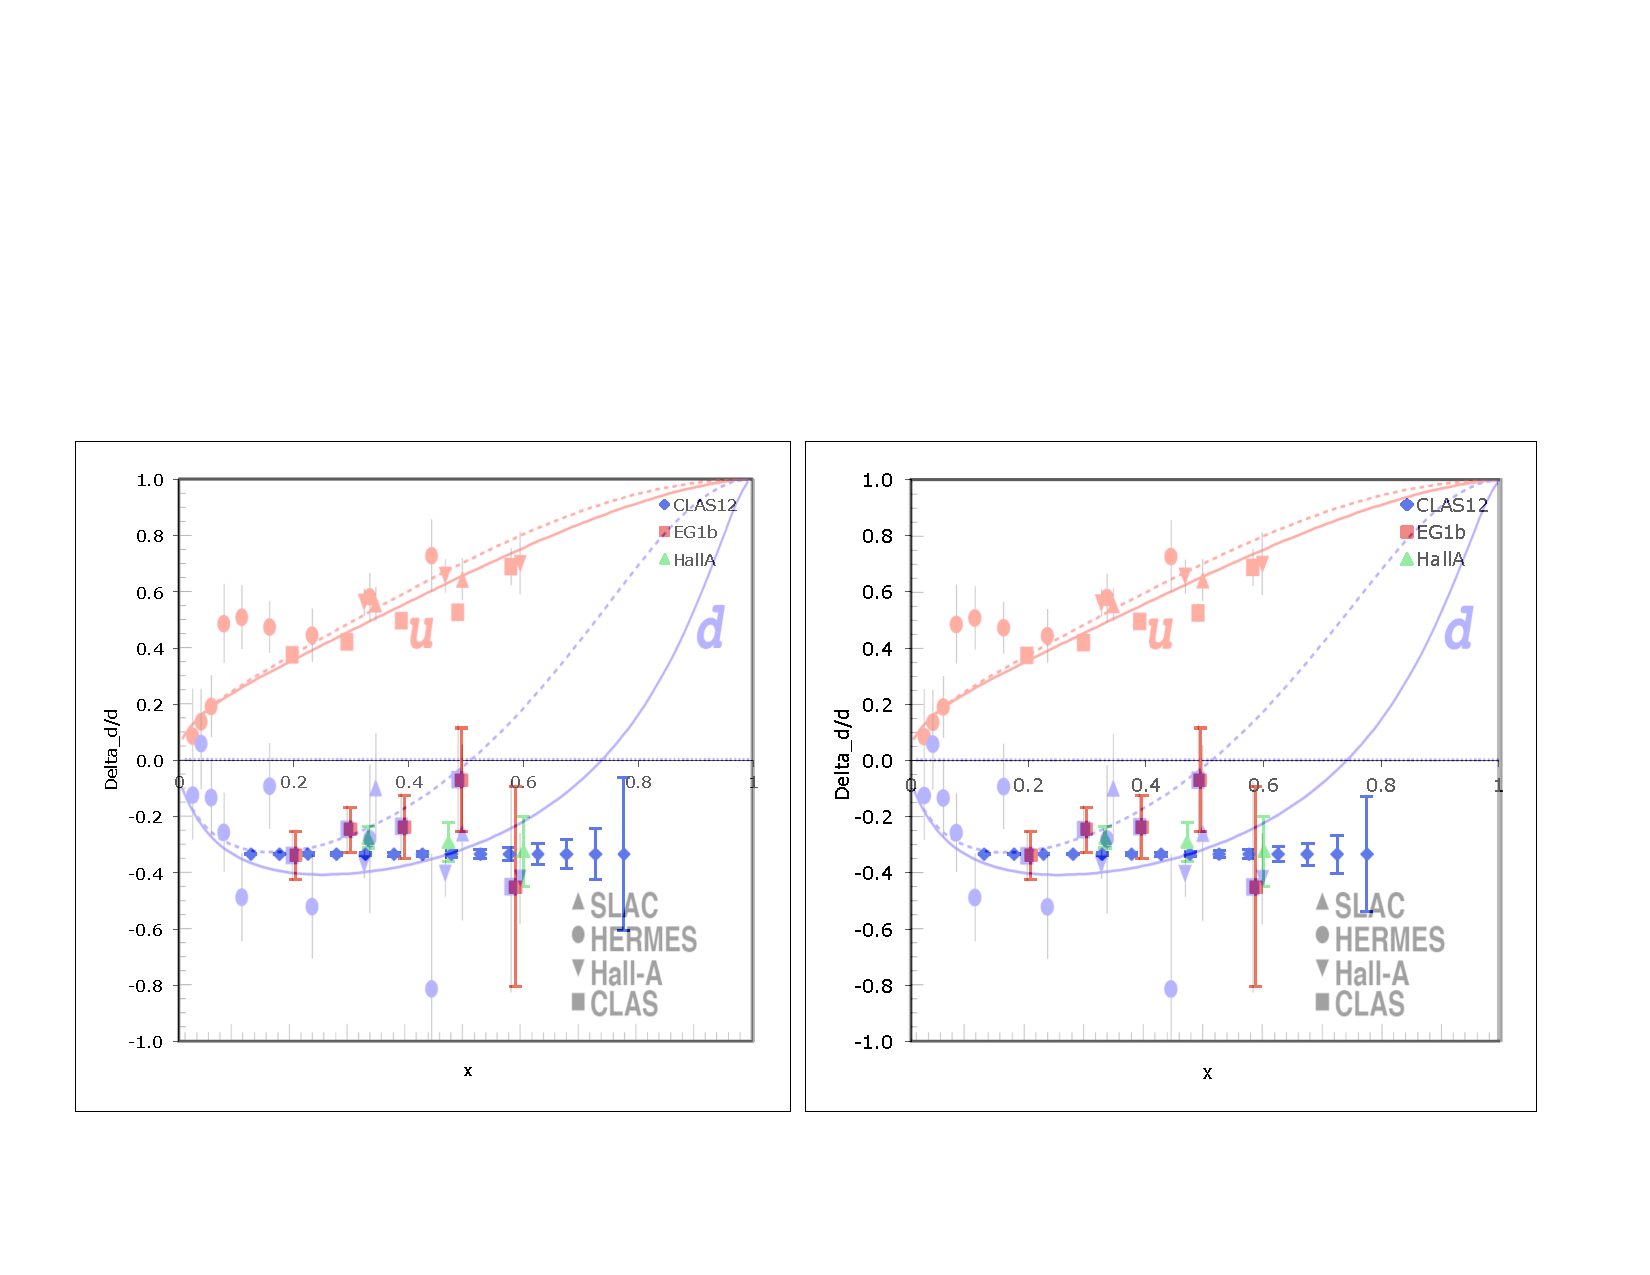
\includegraphics[width=\linewidth]{dis/NewHighX.pdf}
\end{center}
\caption{\baselineskip 13pt \small
Expected statistical precision for the polarization of d quarks, $\Delta d / d$, versus $x$, extracted from E12-06-109 as approved
(l.h.s.) and with an additional 50 days of beam time on the deuteron (r.h.s.). Existing data are shown lightly shaded
(squares are from CLAS at 6 GeV) while the expected data are shown as blue diamonds. The two curves are
the expectations from pQCD without~\cite{Brodsky:1994kg}  and with~\cite{Avakian:2007xa} inclusion of orbital angular momentum effects. The expected data are placed according to expectations from hyperfine-perturbed quark models~\cite{Isgur:1998yb} which,
at least at present, cannot be ruled out.}
\label{highXexp}
\end{figure}

In Figure~\ref{highXexp}, we focus on the impact our proposed data will have on the determination of the d-quark polarization
at the highest $x$ reachable with Jefferson Lab at 12 GeV. The ``expected data points'' are based on a detailed Monte Carlo simulation
of the measured asymmetries on the proton and the deuteron, including both statistical and systematic uncertainties.
While we used a simple-minded LO (``na\"ive parton model'') calculation to extract the valence quark polarizations from these
measurements, the expected uncertainty will not change much with a more sophisticated analysis like the JAM PDF fit 
described above. The obvious point from this figure is that, as presently scheduled, our expected data will have limited
statistical power to definitely answer the question (by themselves) whether $\Delta d / d$ remains negative for $x \rightarrow 1$
as expected from some NLO fits~\cite{Leader:2006xc} and from hyperfine-perturbed quark models~\cite{Isgur:1998yb} or whether it 
will converge to $+1$ as expected by pQCD, as indicated in the solid curves in Fig.~\ref{highXexp}. In particular, the two last
data points are only 3.7 and 1.2 standard deviations from zero, so with a statistical fluctuation of the actually measured data points 
by only one standard deviation, the solid curve in Fig.~\ref{highXexp} would still be (nearly) compatible with those data,
with a $\chi^2$ of 4.9 for two degrees of freedom ($p = 8.7 \%$). 

With a doubling of the integrated luminosity on the deuteron, the statistical error bars on $\Delta d / d$ will go down nearly exactly
by a factor of $1/\sqrt{2}$, since the proton results (that also enter the calculation) are already vastly more precise than the deuteron
ones. As stated above, the systematic uncertainties will also go down, by nearly the same amount (and the uncertainties
 are statistics-dominated
at high $x$). Repeating the same calculation, we find that the agreement with the ``wrong'' curve is now much worse, with
a $\chi^2$ of 11.3 for two degrees of freedom ($p = 0.35 \%$). While it is true that more information on $\Delta d / d$ is expected
from the approved experiments on $^3$He, it is precisely at high $x$ that smearing effects and uncertainties from nuclear binding
become the largest, making an independent measurement on the most lightly bound nucleus, deuterium, mandatory. Our
proposal for an additional 50 days on that target will strengthen this independent result significantly.

\subsection{Further results from SIDIS}

%We request 25 days of highly polarized ($> 85 \%$) electron beam (about 10-20 nA) on a 3 cm long
%NH$_3$ target (80 \% polarization on average) and 45 days on a 3 cm long ND$_3$ target 
%(40 \% polarization on average). In addition, we request 10 days of beam on auxiliary targets
%(carbon - 8 days, and empty - 2 days). We also will need 5 additional days (without beam) for
%target changes, anneals
%(which will be needed about every other day), polarization reversals, and calibrations. The quoted
% parameters are fully consistent with recent operating experience
%during eg1-DVCS, which ran in 2009, including several days on an ND$_3$ target (which exhibited
%a slow drop of its polarization from about 43\% to 33\% during a 2-day period after it received its
%optimal radiation dose). The beam time requests are optimized so that statistical errors will be 
%smaller or comparable to systematic ones in all kinematics of interest. In particular, the running
%time on deuterium is longer to partially compensate for the lower polarization and to
%maximize the impact on NLO extractions of polarized parton densities. In Figs.~\ref{A1eg12}-\ref{rest} 
%we show a few 
%representative results expected from this data set; these as well as additional plots (based on
%a full simulation of CLAS12) are contained in the original proposal.


\begin{figure}[htb!]
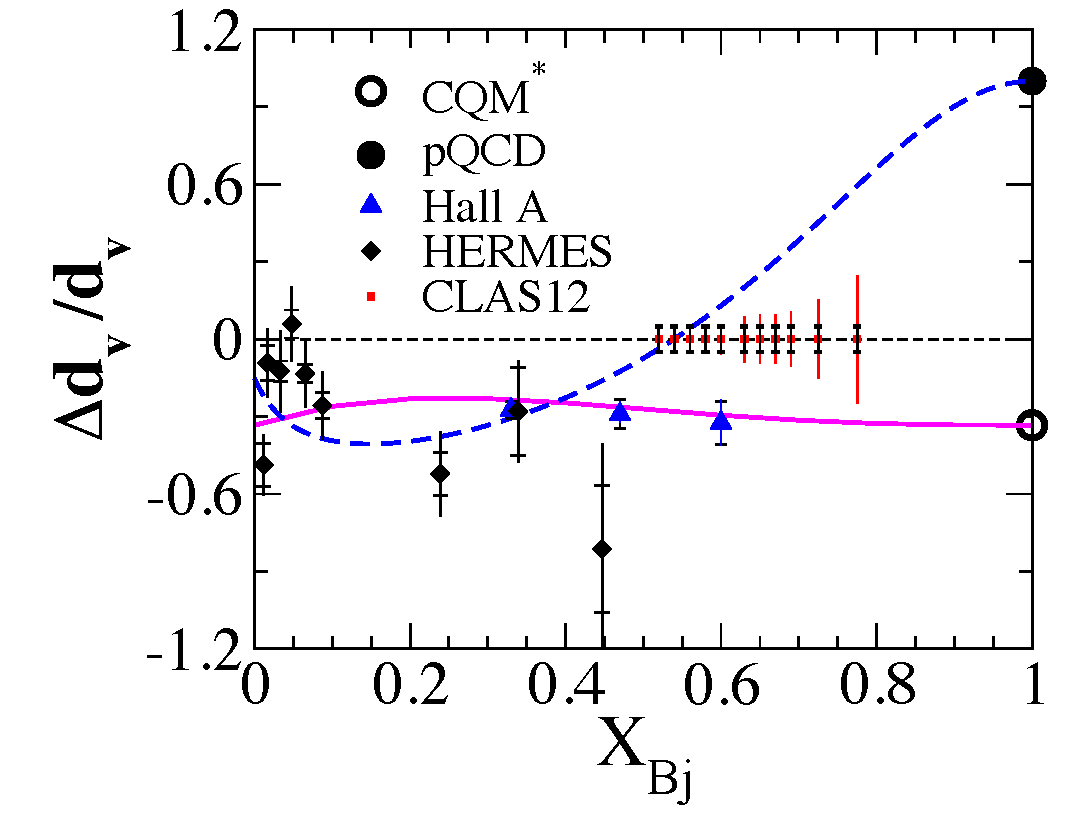
\includegraphics[width=0.66\linewidth]{dis/DeltaDoverD-eps-converted-to.pdf}
%\end{minipage}%\hfill
\caption{\baselineskip 13pt \small
Expected results for the valence $d$ quark polarization from semi-inclusive data
with the proposed experiment, as well
as existing data. The horizontal risers indicate the systematic uncertainties, while the length of the error bars
indicates the statistical uncertainties.
The dashed line represents a pQCD prediction~\cite{Brodsky:1994kg}
 while the solid line represents the prediction from the
  hyperfine perturbed constituent quark model~\cite{Isgur:1998yb}. }
\label{rest}
\end{figure}

In addition to the determination of polarized PDFs from inclusive DIS measurements,  run group C also supports a large number
of approved measurements with semi-inclusive detection of pions and Kaons. For example, we show in Fig.~\ref{rest} the
expected results from a combination of SIDIS production of pions ($\pi^+$ and $\pi^-$) from both proton and deuteron targets
that directly measures (in LO) the valence d-quark polarization. This figure is from the original proposal for E12-06-109
and hasn't been updated yet, but it is clear that similar arguments as for the previous subsection apply: A reduction of the 
statistical error bars (indicated by the {\em full} length of the vertical lines) by a factor $1/\sqrt{2}$ would turn this marginally
significant measurement into a strong, independent confirmation for the trend observed in DIS.

\begin{figure} [!htbp]
\begin{minipage}[t]{0.5\linewidth}
%\epsfxsize=\linewidth
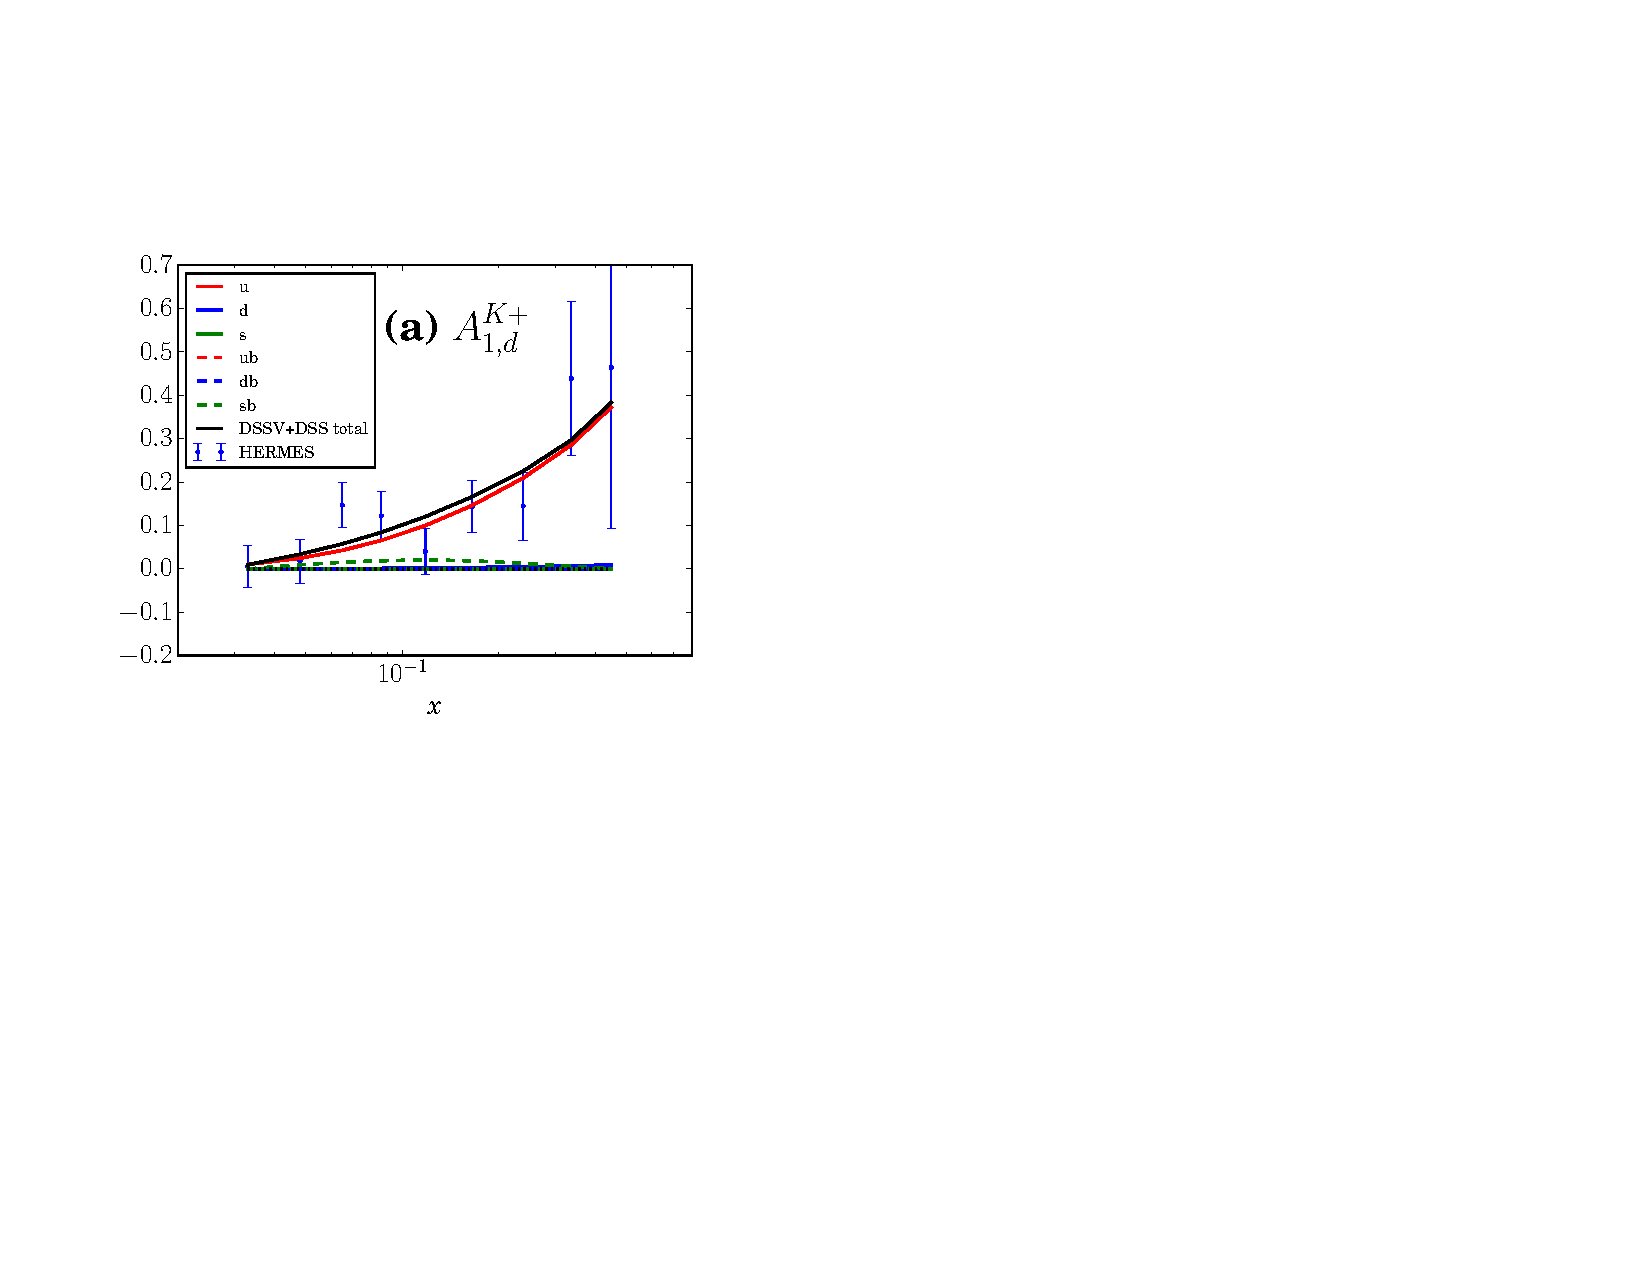
\includegraphics[width=\linewidth]{dis/Kplusd.pdf}
\end{minipage}%\hfill
\begin{minipage}[t]{0.5\linewidth}
%\epsfxsize=\linewidth
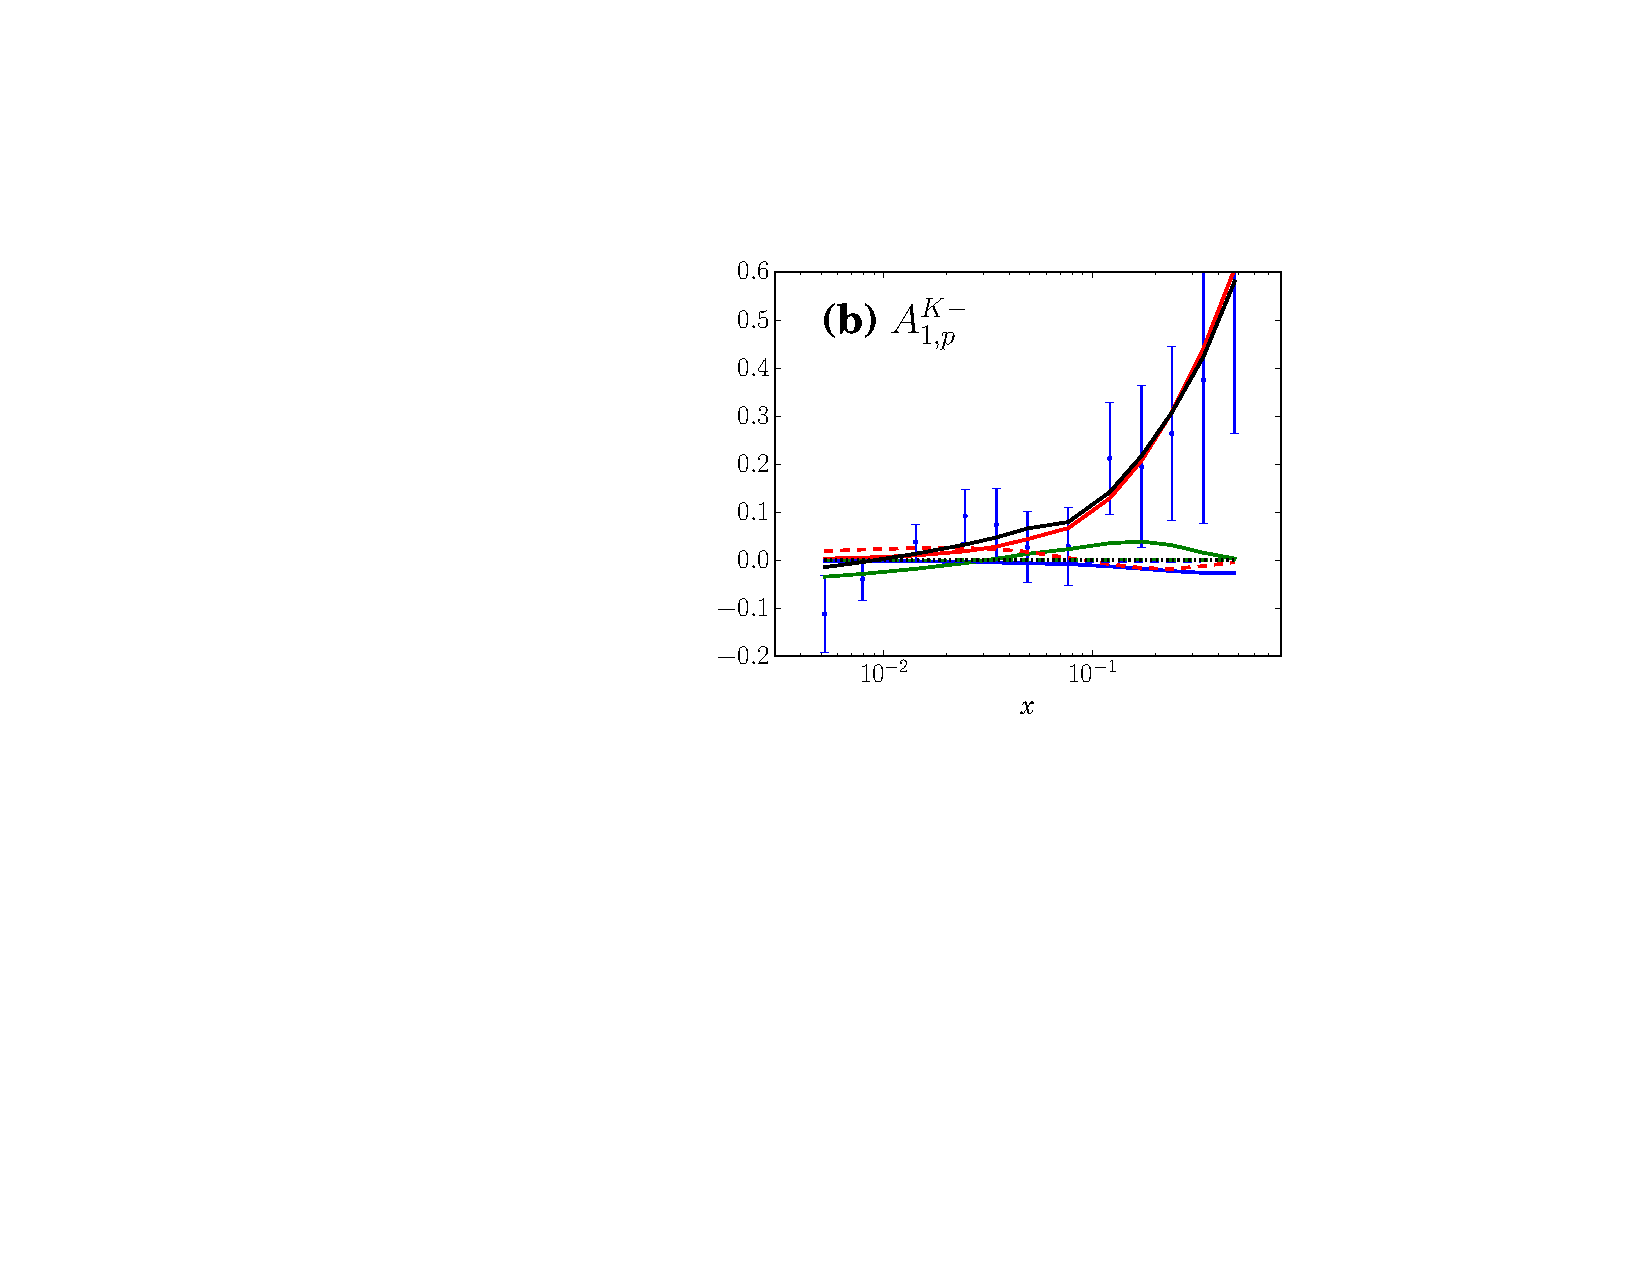
\includegraphics[width=\linewidth]{dis/Kminusp.pdf}
\end{minipage}
\begin{minipage}[b]{\linewidth}
%\epsfxsize=\linewidth
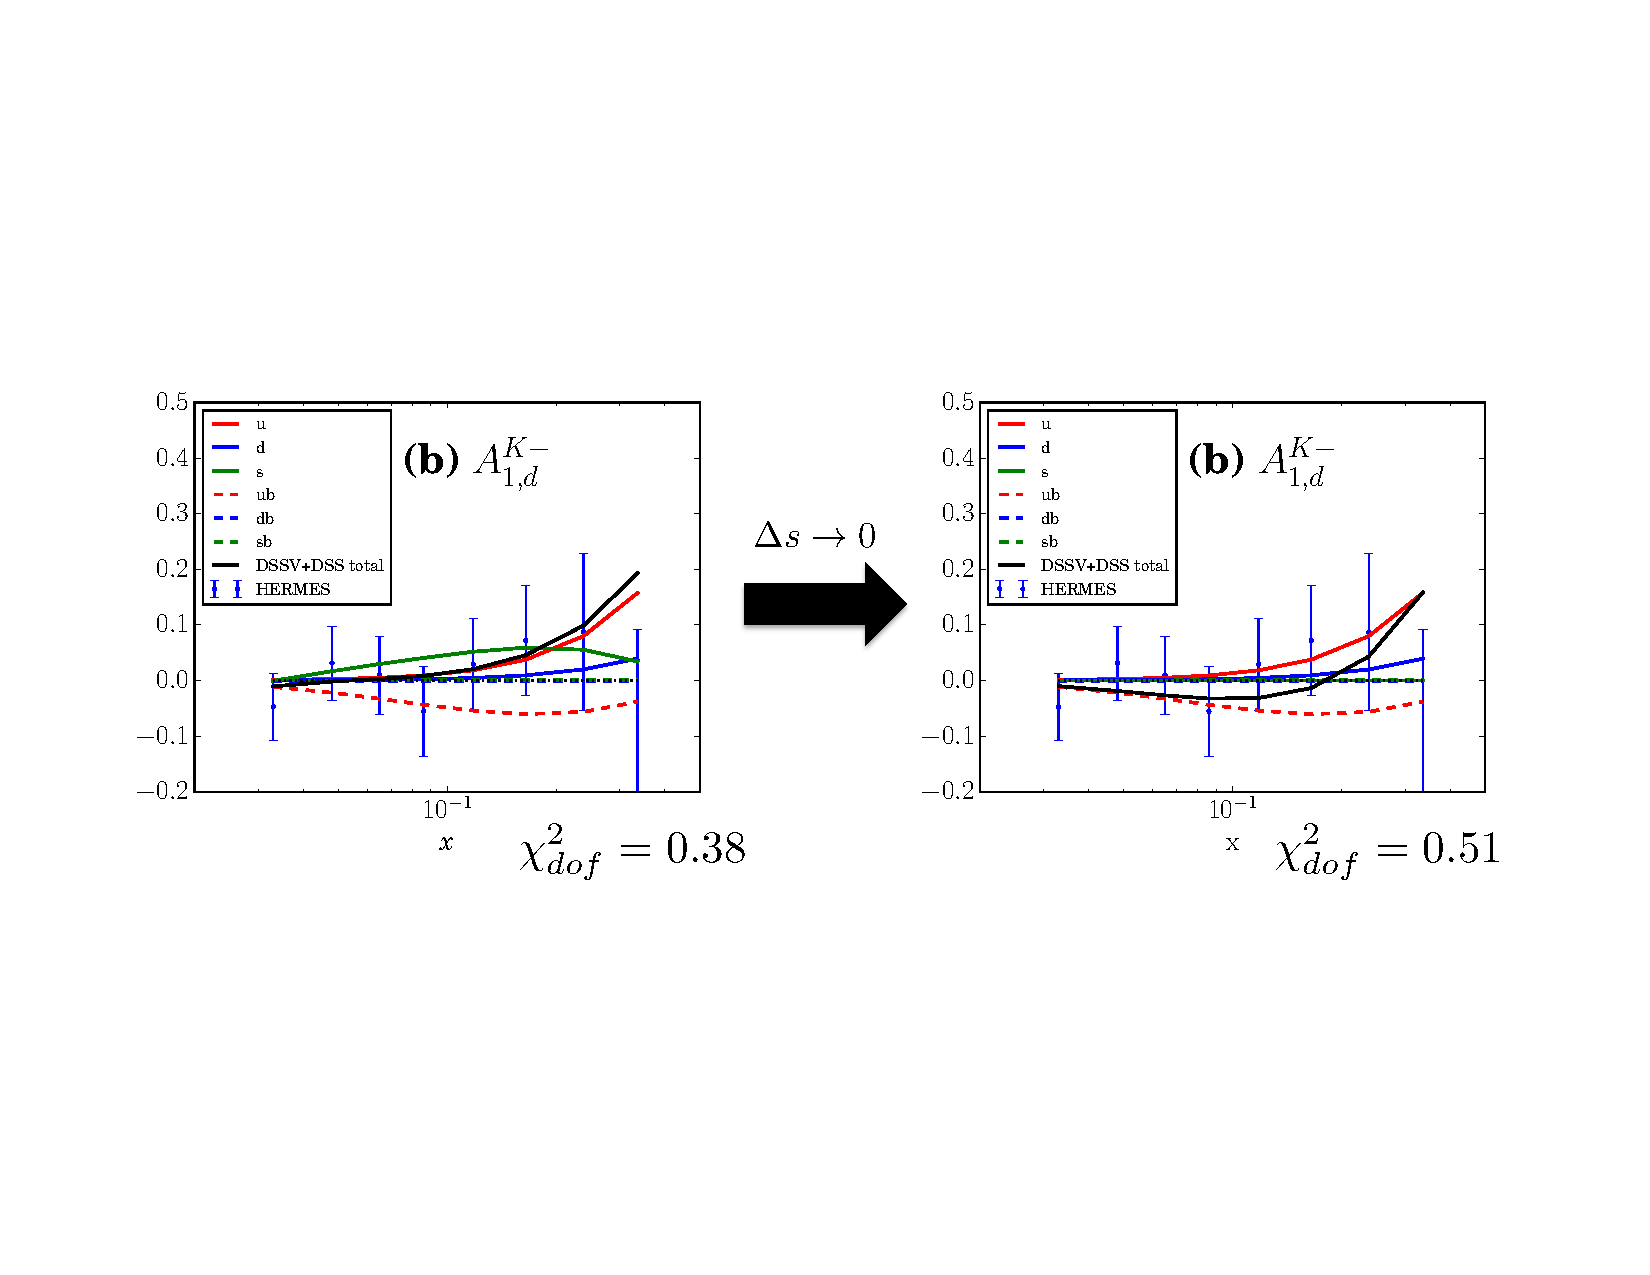
\includegraphics[width=\linewidth]{dis/Kminusd.pdf}
\end{minipage}%\hfill
\caption{\baselineskip 13pt \small
Contributions to the measured asymmetry in SIDIS Kaon production from various quark (solid lines) and
anti-quark (dashed lines) flavors, according to a preliminary JAM
analysis. The data points are from HERMES.
The top row shows  the $K^+$ asymmetry on the deuteron (l.h.s.) and the $K^-$ asymmetry on the proton
(r.h.s.). The bottom row shows two fits to the $K^-$ asymmetry on the deuteron, either with the s-quark contribution
allowed to vary freely for a minimized $\chi^2$ (left) or with this contribution set to zero (right). Figure courtesy of J.J. Ethier. }
\label{kaon}
\end{figure}

More generally, a combined analysis of all inclusive and semi-inclusive measurements within the framework of NLO DGLAP
analysis will further constrain the individual quark and gluon PDFs and allow a clear separation of quark and antiquark
contributions of each flavor to the sea. The JAM collaboration is now gearing up to include this information in their fits,
carefully assessing the impact of our (lack of) knowledge of the required fragmentation functions. While simulations are not
yet available, it is clear again that higher precision will translate in additional knowledge. As an example we consider
(in Fig.~\ref{kaon}) the impact of various measurements on our knowledge of the strange quark sea in the nucleon, which
is still a contentious topic without a clear consensus whether the contribution of this strange sea to the nucleon spin is
positive, negative or negligible.

The top row of Fig.~\ref{kaon} shows that the $K^+$ asymmetry (on either target) and the $K^-$ asymmetry on the proton are rather insensitive
to the strange quark polarization, since in both cases u-quarks dominate because of their prevalence and larger charge.
However, the $K^-$ asymmetry on the deuteron is much more sensitive to strange quarks, since in the deuteron,
u and d quark contributions to $K^-$  production fortuitously cancel to a large extent. Hence, a precise measurement of
this channel down to the lowest available $x \approx 0.06$ at Jefferson Lab has great promise to answer the question whether
strange quarks in the nucleon carry positive helicity, negative helicity or whether there is a node in the distribution where
their polarization transitions from plus to minus.
Unfortunately, the only data existing so far (from HERMES) have large error bars, so that an alternative fit without any
s-quark contribution only increases the $\chi^2$ per degree of freedom from 0.38 to 0.51 (see bottom row of Fig.~\ref{kaon}).
With the vastly better statistics available from CLAS12, this situation should be much improved (note that CLAS12
will cover the same kinematic region as HERMES except for the two lowest data points). The importance of
finally ``nailing down'' this least-known quark contribution to the nucleon spin is another strong justification to collect
the highest statistics data set on the deuteron possible.

\section{Beam Request}

We request 50 additional days, for a total of 100 days, of 11 GeV longitudinally polarized ($> 85 \%$) electrons on a longitudinally polarized ND$_3$ target in CLAS12, plus 23 additional days for calibration, in-situ irradiation of the target material, target changes, anneals and polarization reversals, as well as beam polarization (M\o ller) measurements. 
The additional 10 days at 5 nA with the inclusion of the FT, as requested in the nDVCS part of this proposal, will not directly impact the program of measuring collinear spin structure functions and has not been included in the estimates that were presented in this chapter. However, it offers the potential for measurements of spin structure functions at very low $Q^2$ that are of interest in their own right, and as part of the radiative corrections for DIS.
